\chapter{Doppler frequency-based satellite-aided positioning}
% todo rearrange whole section
% todo change intro
As outlined in section \ref{s_int_doppler_shift_method}, the three principal steps in determining a user position from Doppler frequency measurements of a satellite signal are: determining the identity and position (or trajectory) of the transmitting satellite, acquiring and tracking the transmitted signal and measuring its frequency, calculating the user position from the measured data and compensating errors. 

These three steps can be further broken down to:
\begin{enumerate}
    \item identifying the transmitting satellite,
    \item determining the position or trajectory of the transmitting satellite,
    \item acquiring the transmitted signal,
    \item tracking the transmitted signal,
    \item measuring the frequency of the transmitted signal,
    \item calculating the user position from the measured data,
    \item estimating and compensating the errors introduced in each of the previous steps.
\end{enumerate}

This chapter first describes the Doppler frequency-based method, henceforth referred to as the \emph{Doppler method}, and then goes through the steps of its realisation, thus laying the groundwork for the system designed in this work.

\section{Doppler effect}
The Doppler effect is the change in the frequency of a wave as perceived by an observer who is moving relative to the source of the wave. The received frequency can be expressed as
\begin{equation*}
    f_R = \frac{c + v_R}{c - v_T} f_0
\end{equation*}
 where $c$ is the speed of wave in the medium, $v_R$ and $v_T$ are the respective velocities of the receiver and transmitter relative to the medium (positive direction is toward each other), and $f_0$ is the transmitted frequency. For a stationary receiver ($v_R = 0$) it can be simplified to
 \begin{equation}
 \label{e_pos_doppler}
    f_R = \frac{c}{c - v_T} f_0
\end{equation}
Further simplification yields the original frequency:
 \begin{equation}
 \label{e_pos_doppler_f0}
    f_0 = f_R (1 - \frac{v_T}{c})
\end{equation}


\section{The Doppler method}
\label{s_pos_doppler_method}
% todo doppler method intro
 

\subsection{An ideal case}
First, a ideal-case example is discussed (see fig. \ref{f_pos_doppler_method_simple}) to illustrate the method.

\begin{figure}
    \centering
    \includegraphics[width=0.75\linewidth]{img/pos_doppler_method_simple}
    \caption{The Doppler method (ideal case)}
    \label{f_pos_doppler_method_simple}
\end{figure}

A satellite passes on a circular trajectory over the surface of the Earth with a tangential velocity $v$, transmitting a signal on a frequency $f_0$. On the surface, a user measures a Doppler-shifted frequency $f_R$.

The Doppler shift can be expressed as
\begin{align}
    f_D &= f_R - f_0 \\
    \textnormal{substituting eq. \ref{e_pos_doppler_f0}: } 
    f_D &= f_R - f_R (1 - \frac{v_T}{c}) \\
    \textnormal{simplified as } 
    f_D &= f_R \frac{v_T}{c} \label{e_pos_dopp_shift}
\end{align}

The velocity $v_T$ is a relative speed of the satellite to the user. Its direction is from the satellite to the user, and it is offset from the satellite velocity by the angle $\alpha$. It can be expressed as
\begin{equation*}
    v_T = v \ \cos{\alpha}
\end{equation*}
Thus, the Doppler shift can be expressed as
\begin{equation}
    \label{e_pos_fd}
    f_D = f_R - f_0 = f_R \frac{v}{c} \cos{\alpha}
\end{equation}

The only parameter which relates the position of the satellite and the user is the angle $\alpha$. It is expressed from the above as
\begin{equation}
    \label{e_pos_cos_alpha}
    \cos{\alpha} = \frac{f_R - f_0}{f_R \ v \ c^{-1}}
\end{equation}

The user is located somewhere on an infinite cone with the centre at the position of the satellite at the time of measurement, the axis in the direction to $v$ and an opening angle $2\alpha$.

If this measurement is carried out several times at a different satellite positions along its trajectory, the user position can be pinpointed to the intersections of the respective cones. Additionally, if the user is assumed to be on the surface, an intersection with a sphere representing the surface can be considered.

However, for a pass of a single satellite, the Doppler method always yields at least two results (one actual and one shadow) symmetrical along the satellite ground track (see fig, \ref{f_pos_doppler_symmetry_problem}). Additional satellite measurements or other means are necessary to resolve the symmetry problem and determine which position is the correct one.

\begin{figure}
    \centering
    \includegraphics[width=0.75\linewidth]{img/pos_doppler_symmetry_problem}
    \caption{Illustration of the Doppler method symmetry problem\cite{sop09}}
    \label{f_pos_doppler_symmetry_problem}
\end{figure}


\section{Acquiring the satellite signal}
Provided the transmission frequency of the satellite is known, either exactly or by a set or a range, the signal can be acquired. However, the signal received will be shifted from the original frequency due to the Doppler effect. Knowledge of the bounds of this shift is critical for acquiring the satellite signal.

The largest shift occurs when $\cos{\alpha} = 1$ in eq. \ref{e_pos_fd}, that is, when the satellite radius vector is perpendicular to that of the receiver. However, in this situation, the satellite in LEO is invisible to the receiver. More practically, the largest Doppler shift occurs when the satellite is first (and last) visible to the receiver. For a ground-based receiver with no obstacle in sight, this happens when the satellite intersects a plane tangential to the Earth surface at the receiver position (see fig. \ref{f_pos_max_doppler_shift}).

\begin{figure}
    \centering
    \includegraphics[width=0.75\linewidth]{img/pos_max_doppler_shift}
    % TODO actual figure
    \caption{Situation for maximum Doppler shift}
    \label{f_pos_max_doppler_shift}
\end{figure}

In this special case, the angle $\alpha$ is equal to the angle $\gamma$ between the satellite and user radius vectors. Thus,
\begin{equation*}
    \cos{\alpha} = \frac{R_E}{R_E + h}
\end{equation*}
where $R_E$ is the radius of the Earth and $h$ is the orbital altitude of the satellite.

Orbital velocity for a circular orbit is approximately
\begin{equation*}
    v \approx \sqrt{\frac{\mu}{R_E + h}}
\end{equation*}
where $\mu$ is the standard gravitational parameter. Thus, substituting the above into eq. \ref{e_pos_fd}, the maximum Doppler shift depends only on the orbital altitude and transmission frequency:
\begin{equation}
    \label{e_pos_fd_max}
    f_{D max} \approx f_R \frac{1}{c} \sqrt{\frac{\mu}{R_E + h}} \frac{R_E}{R_E + h}
\end{equation}

The maximum Doppler shift for the satellites considered in the LEO system survey in section \ref{s_sat} is in table \ref{t_pos_max_fd}.

\begin{table}
    \centering
    \begin{tabular}{llll}
    System     & $h$ (km) &  $f_R$ (MHz) & $f_{Dmax}$ (kHz) \\ \hline
    Iridium    &  781  &  1626 & \num{36.1} \\
    Orbcomm    &  715  &  138  & \num{3.1} \\
    Globalstar &  1414 &  2500 & \num{48.9}
    \end{tabular}
    \caption{Maximum Doppler shift for select LEO satellites}
    \label{t_pos_max_fd}
\end{table}

\section{Calculating user position}
A review of existing work reveals three main ways of using the Doppler shift method.

The first method is the one used by the Transit navigation system, based on creating a trial Doppler curve from an estimated location and fitting it to the measured curve, thus calculating the actual location\cite{sat16}.

The second method is geometrical. It is based on an intersection of three surfaces - a sphere defined by a model of the surface of the Earth, a cone defined by a constant range rate (see cone in Fig. \ref{f_pos_doppler_method_simple}), and a sphere one defined by a constant range to the satellite\cite{sop22}. Since range measurements are not available in this work, the range sphere must be substituted by another surface, such as a second range-rate cone.

The third method is the most common in the reviewed modern research. It is based on expressing a the range rate as a function of measured frequency and as a function of satellite position and velocity and user position. These are then equated and the user position is found\cite{sop02, sop13}.

All three methods are explained in detail below.

\subsection{The Doppler curve fitting method}
\label{s_transit_nav_method}
The Doppler curve fitting method is based on measuring the frequency emitted by a satellite, thus obtaining a Doppler shift curve, and then retroactively determining (2D) user location.

The user latitude is determined by the moment when the received frequency is equal to the transmitting frequency, as in that moment the satellite range rate is zero. Thus, the user is located on a plane perpendicular to the satellite orbital velocity. The Transit satellites were on a polar orbit, therefore at the moment of zero range rate the satellite is at an equal latitude as the user.

The user longitude is determined by the shape of the Doppler curve. The rate of change of Doppler frequency is the largest if the satellite passes directly overhead and smallest if the satellite passes over the horizon, as are the minima and maxima of the received frequency. The rotation of the Earth provides another part in the relative motion of the satellite and the user, and can be used to determine whether the satellite passes to the west or the east of the user.

A trial Doppler curve is calculated based on an initial estimate of user position, and it is compared to the actual measured curve using a least-squares fit. The estimate of the user position is then updated and the process iterated, until the two curves match\cite{sat16}.


\subsection{The surface intersection method}
% todo section from sop22


\subsection{The range rate method}

\begin{equation}
    f_D = \frac{\dot\rho f_R}{c}
\end{equation}

\begin{equation}
    \dot\rho_i = \frac{c f_{D_i}}{f_R}
\end{equation}

\begin{equation}
    \dot\rho_i = (V_i - V) \frac{r_i - r_0}{||r_i - r_0||^2} + c \dot\delta t - c \dot \delta t^i + v
\end{equation}


\begin{equation}
    \frac{c f_{D_i}}{f_R} = (V_i - V) \frac{r_i - r_0}{||r_i - r_0||^2} + c \dot\delta t - c \dot \delta t^i + v
\end{equation}


\section{Satellite position}
\label{s_pos_tle_sgp4} 
The Doppler method requires the knowledge of the position of the transmitting satellite, which is then used as a reference. Unless the satellite itself transmits its position (which is the case for Iridium Ring Alert messages, albeit in a low resolution), the position needs to be calculated on the user side. To do this, the satellite orbit needs to be known and a propagation model used to calculate the satellite position at a given time.

A widely used approach utilises Two Line Element (TLE) sets, which contain orbital parameters for satellites, and the Simplified General Perturbations-4 (SGP4) model for propagation. TLEs are regularly updated by the North American Aerospace Defense Command (NORAD) and are publicly available via e.g. the CelesTrak project website\cite{des11}. An analysed example of TLE is shown in \autoref{f_pos_tle}. A TLE is valid for a given time, called an \textit{epoch}.

\begin{figure}
    \centering
    \includegraphics[width=1\linewidth]{img/pos_tle.PNG}
    \caption{Structure of a TLE set\cite{pos06}}
    \label{f_pos_tle}
\end{figure}

The SGP4 model is an orbit propagation model developed by the U.S. Air Force in the 1960s and further refined e.g. by Vallado et al.\cite{des06}. It is compatible with TLEs and commonly used together. The perturbation calculations are simplified - the Earth’s gravitational model is truncated, the atmospheric model is a static density field with exponential decay, and third-body influences are modelled only partially\citep{pos01}{698}. The SGP4 model works in the TEME coordinate frame (see \autoref{s_pos_frames_of_ref}).

The accuracy of the model was evaluated in \cite{pos07}, which concluded that for the satellite constellations under evaluation in this work the position prediction errors one day from TLE epoch are on the order of \qty{e2}{m}, with maximum errors between \qtyrange{3}{6}{km}, depending on the intensity of the Solar flux.


\section{Frames of reference}
\label{s_pos_frames_of_ref}
Any position needs to be expressed in a frame of reference. For terrestrial calculations, it is advantageous to use an Earth-centred frame, which has its origin at some centre (e.g. gravitational, physical) of the Earth. There are two general types of Earth-centred frames: Earth-Centred Inertial (ECI), which are fixed relative to some position external to the Earth (usually the Earth's position at equinox) and thus do not rotate with the Earth (they are inertial), and Earth-Centred Earth-Fixed (ECEF), which are fixed to a point on Earth and thus do rotate with it (they are non-inertial).

For this work, three frames of reference are important: TEME (ECI), ITRS (ECEF) and WGS84 geodetic datum (ECEF).

The process of transforming between those systems is described e.g. in \cite{pos01}, and the transformations used in this work are all based on the equations and algorithms provided there: from TEME to ITRS \citep{pos01}{231-233}, from ITRS to geodetic \citep{pos01}{174-179} and back \citep{pos01}{146}.

\subsection{True Equator Mean Equinox}
The True Equator Mean Equinox (TEME) reference frame is a Cartesian ECI frame. The z-axis points along the Celestial Ephemeris Pole\footnote{The Earth rotation axis} (CEP), while x-axis is located on the True Equator plane (a plane perpendicular to the CEP) and points in the direction of the Vernal Equinox without accounting for celestial nutation (the \textit{mean} or \textit{uniform} equinox)\citep{pos01}{231-233}. TEME frame is used by the SGP4 algorithm (see \autoref{s_pos_tle_sgp4}).

\subsection{International Terrestrial Reference System}
The International Terrestrial Reference System (ITRS) is a standard Cartesian ECEF frame. The origin is at the centre of mass of the Earth and the axes are fixed to defining coordinates on Earth. As a result of tectonic movement, the system is periodically recalculated\citep{pos01}{152}. All calculations within this work are done in ITRS.

\subsection{World Geodetic System Geodetic Datum}
The World Geodetic System-84 (WGS84), where 84 refers to the most recent version from 1984, is an ECEF frame maintained by the U.S. National Geospatial-Intelligence Agency. The WGS84 and ITRS agree on a level of \unit{cm}\citep{pos01}{203}. The geodetic datum  (hereafter referred to as only \textit{geodetic frame}) is a latitude-longitude-altitude ($\phi, \lambda, h$ respectively) frame defined within WGS84. In this work, the estimated position is in the geodetic frame for clarity, however, for navigation calculations themselves the position is always converted to ITRS.

\section{Capturing a satellite signal}
\label{s_pos_tracking_satellite}
One of the basic principles of capturing a satellite signal burst, extensively used in the reviewed literature, is based on thresholding the signal power level.

First, the raw captured signal is amplified by a low noise amplifier (LNA) and is squared once or twice (2\textsuperscript{nd} or 4\textsuperscript{th} power) to increase the prominence of dominant peaks. Then, the Fourier transform (FFT) or a Power Spectral Density (PSD) function is applied with a windowing function (e.g. Hamming or Blackman-Harris). The resultant spectrum is then compared to a threshold representing the noise level. Peaks whose power level is stronger than the threshold and whose frequency falls within the plausible range for the given signal type are considered to be indicative of a present signal. The peak rise and fall times are noted (usually in terms of sample number rather than seconds). 

The samples within those times enter a Phase Lock Loop (PLL) to refine the frequency estimate. The PLL is is composed of a Numerically Controlled Oscillator
(NCO), integrator functions, phase detector and a loop filter. A typical setup is shown in the block diagram in \autoref{f_pos_tracking_block}\cite{sop03, sop04, sop05}.

\tikzstyle{block} = [rectangle, rounded corners, minimum height=1cm, text centered, text width=1cm, draw=black]
\tikzstyle{sum} = [draw, circle, minimum size=0.6cm, fill=black!15]
\tikzstyle{empty} = [draw=white, circle, minimum size=0.6cm, ]
\tikzstyle{arrow} = [thick,->,>=stealth]

\begin{figure}
\centering
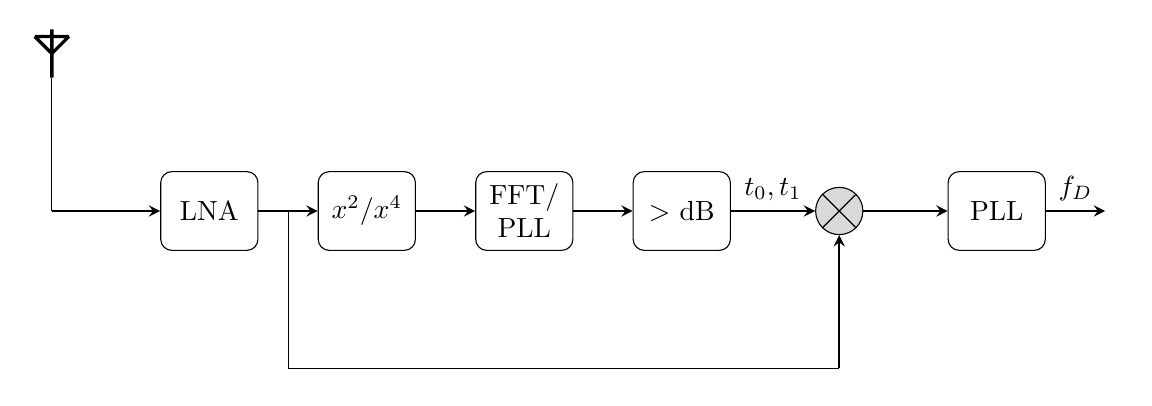
\begin{tikzpicture}[node distance=2cm]

% Sum shape
\node (ant) [empty]{};
\draw [very thick] (ant.north east) -- (ant.center)
      (ant.north west) -- (ant.center)
      (ant.north east) -- (ant.north west)
      (ant.north) -- (ant.south);
\node (antb) [below of=ant]{};
\node (lna) [block, right of=antb] {LNA};
\node (pwr) [block, right of=lna] {$x^2$/$x^4$};
\node (fft) [block, right of=pwr] {FFT/ PLL};
\node (thr) [block, right of=fft] {$>$ dB};
\node (sm1) [sum,   right of=thr]{};
\draw (sm1.north east) -- (sm1.south west)
      (sm1.north west) -- (sm1.south east);
\node (pll) [block, right of=sm1] {PLL};
\node (pllr)  [right of=sm1, xshift=1.5cm]{};

\draw (ant) -- (antb.center);
\draw [arrow] (antb.center) -- (lna);
\draw [arrow] (lna) -- (pwr) node[midway](bypass){};
\draw [arrow] (pwr) -- (fft);
\draw [arrow] (fft) -- (thr);
\draw [arrow] (thr) -- (sm1) node[midway,above]{$t_0, t_1$};
\draw [arrow] (sm1) -- (pll);
\node (sm1b) [below of=sm1]{};
\node (lnab) [below of=bypass]{};
\draw (bypass.center) -- (lnab.center);
\draw (lnab.center) -- (sm1b.center);
\draw [arrow] (sm1b.center) -- (sm1);
\draw [arrow] (pll) -- (pllr) node[midway,above]{$f_D$};
\end{tikzpicture}
\caption{General process of capturing a satellite signal}
\label{f_pos_tracking_block}
\end{figure}